\newcommand{\naive}{na\"{\i}ve}
\newcommand{\dartfmt}{\texttt{dartfmt}}
\newcommand{\gofmt}{\texttt{gofmt}}
\newcommand{\rfmt}{\texttt{rfmt}}
\section{Background}
This chapter explains the necessary background to understand Scala and code formatting.
More specifically, we motivate why Scala presents an interesting challenge for code formatters.
We go into details on Scala's rich syntax and popular idioms that introduced unique challenges to the design of scalafmt.
We follow up with a history on code formatters that have been developed over the last 70 years.
We will see that although code formatters have a long history, a new tradition of optimization based formatters -- which scalafmt proudly joins -- started only recently in 2013.
% Scalafmt follows this new tradition.

\subsection{Scala the programming language}\label{sec:scala}
Scala\autocite{odersky_scala_2004} is a general purpose programming language that was first released in 2004.
Scala combines features from object-oriented and functional programming paradigms, allowing maximum code reuse and extensibility.

Scala can run on multiple platforms.
Most commonly, Scala programs compile to bytecode and run on the JVM.
With the releases of Scala.js\autocite{doeraene_scala.js_2015}, JavaScript has recently become a popular target platform for Scala developers.
Even more recently, the announcement of Scala Native\autocite{_scala-native/scala-native_????} shows that LLVM may become yet another viable target platform for Scala developers.

Scala is a popular programming language.
The Scala Center --- a not-for-profit organization focused on Scala open-source and education --- estimates that more than half a million developers use Scala\autocite{odersky_scala_2016}.
Large organizations such as Goldman Sachs, Twitter, IBM and Verizon rely on Scala code to run business critical applications.
The 2015 Stack Overflow Developer Survey shows that Scala is the 6th most loved technology and 4th best paying technology to work with\autocite{_stack_????}.
The popularity of Apache Spark\autocite{_apache_????-1}, a cluster computing framework for large-scale data processing, has made Scala a language of choice for many developers and scientists working in big data and machine learning.

Scala is a programming language with rich syntax and many idioms.
The following chapters discuss in detail several prominent syntactic features and idioms of Scala.
Most importantly, we highlight coding patterns that encourage developers to write a single large statement over of multiple small statements.

\subsubsection{Higher order functions}
Higher order functions (HOFs) are a common concept in functional programming languages as well as mathematics.
HOFs are functions that can take other functions as arguments and return functions as values.
Languages that provide a convenient syntax to manipulate HOFs are said to make functions first-class citizens.

Functions are first-class citizens in Scala.
Consider listing~\ref{lst:hof}.
\lstinputlisting[label={lst:hof}, float, caption=Higher order functions]{code/hof.scala}
The method \texttt{twice} takes an argument \texttt{f}, which is a function from an integer to an integer.
The method returns a new function that will apply \texttt{f} twice to an integer argument.
This small example takes advantage of several syntactic conveniences provided by Scala.
For example, in line 2 the argument \texttt{\_ + 3} creates a new \texttt{Function[Int, Int]} instance.
The function call \texttt{f(x)} is in fact sugar for the method call \texttt{f.apply(x)} on the \texttt{Function[Int, Int]} instance.
Listing~\ref{lst:hof_nosugar} shows an equivalent program to listing~\ref{lst:hof}, without using syntactic conveniences.
\lstinputlisting[label={lst:hof_nosugar}, float, caption=Higher order functions expanded]{code/hof-nosugar.scala}
Observe that the body of \texttt{twice} was expressed as a single statement in line 1 of listing~\ref{lst:hof} but as two independent statements in listing~\ref{lst:hof_nosugar}.

\subsubsection{Term blocks}
Scala allows term blocks to appear anywhere in a Scala code.
A term block is a sequence of statements wrapped by curly braces \texttt{\{\}}.
Listing~\ref{lst:block} shows two examples of term blocks.
\lstinputlisting[label={lst:block}, float, caption=Term blocks]{code/block.scala}
Variables bounds inside a term block do not escape the block.
Therefore, the variable \texttt{y} can be assigned both inside the first block as well as to the return value of the \texttt{function} call.
The lightweight syntax to create term blocks in Scala make them a popular feature among Scala developers.
Observe that without term blocks, the second argument to \texttt{function} would be defined externally.
Instead, the second argument is defined inline making the entire \texttt{function} call significantly bigger.

% Blocks are .
% \subsubsection{Immutability}
% Functional programming encourages stateless functions which operate on immutable data structures and objects.
% An immutable object is an object that once initialized, cannot be modified.
% Immutability offers several benefits to software development in areas including concurrency and testing.
% Listing~\ref{lst:immutable} shows an example of manipulating an immutable list.
% \lstinputlisting[label={lst:immutable}, float, caption=Manipulating immutable list]{code/immutable.scala}
% Note that each \texttt{map} and \texttt{filter} operation creates a new copy of the list with the modified contents.
% The original list remains unchanged.
% Listing~\ref{lst:mutable} show the equivalent operation using a mutable list.
% \lstinputlisting[label={lst:mutable}, float, caption=Manipulating mutable list]{code/mutable.scala}
% Observe that listing~\ref{lst:immutable} is a single statement while listing~\ref{lst:mutable} contains multiple statements.

\subsubsection{SBT build configuration}\label{sec:sbt}
SBT\autocite{_sbt_????} is an interactive build tool used by many Scala projects.
SBT configuration files are written in \texttt{*.sbt} or \texttt{*.scala} files using Scala syntax and semantics.
Although SBT configuration files use plain Scala, they typically use coding patterns which are different from traditional Scala programs.
Listing~\ref{lst:sbt} is an example project definition in SBT.
\lstinputlisting[label={lst:sbt}, float, caption=SBT project definition]{code/sbt.scala}
Observe that the project is defined as a single statement and makes extensive use of symbolic infix operators.
Due to the nature of build configurations, argument lists to can becomes unwieldy long and a single project statement can span over dozens or even hundreds of lines of code.


\subsection{scala.meta}\label{sec:scalameta}
Scala.meta\autocite{scala57:online} is a metaprogramming toolkit for Scala.
Before scala.meta, most metaprogramming facilities relied on Scala compiler internals.
This had several severe limitations such as too-eager desugaring resulting in loss of syntactic details from the original source code.
Scala.meta was designed to overcome these limitations and offer a more robust platform to develop metaprogramming tools for Scala.
Several key features of scala.meta have made it an invaluable companion in the development of scalafmt.
Most notably among these features are dialect agnostic syntax trees, syntax tree serialization, high-fidelity  parsing and algebraically typed tokens.

Scala.meta provides facilities to tokenize and parse a variety of different Scala dialects.
One such dialect is SBT configuration files, discussed in section~\ref{sec:sbt}.
SBT adds custom support for top-level statements in \texttt{*.sbt} files, a disallowed feature in regular Scala programs.
Working around this issue requires either depending on the SBT parser or reimplementing its parsing logic.
To add insult to injury, top-level statements must be separated by a blank line if you use an SBT version 0.13.6 or lower; a restriction that was lifted in SBT 0.13.7.
Listing~\ref{lst:dialect} show how to scala.meta makes it trivial to accommodate this zoo of nuances.
\lstinputlisting[label={lst:dialect}, float, caption=Parsing different Scala dialects with scala.meta]{code/dialect.scala}
The result after parsing is a dialect agnostic scala.meta tree structure.

The structure of scala.meta trees can be serialized to strip off all insignificant syntactic details.
Listing~\ref{lst:structure} shows how to serialize the tree structure of a simple hello world application.
\lstinputlisting[label={lst:structure}, float, caption=Serializing scala.meta trees]{code/structure.scala}
For example, observe that the comment has been stripped away.
As we discuss in section~\ref{sec:tooling}, this feature was instrumental in testing scalafmt.

Tree node types in scala.meta preserve absolute fidelity with the original source file.
This means we can obtain all syntactic details from a tree node such as whether a for comprehension uses parentheses or curly braces as delimiters, whitespace positions, comments and other syntactic trivia.
The Scala compiler is infamous for desugaring for-comprehensions into \texttt{map/withFilter/flatMap} applications during the parse phase.
This made it impossible to implement metaprogramming tasks such as code formatting.
High-fidelity parsing in scala.meta has been essential for scalafmt because we can't lose critical syntactic details such as whether for-comprehensions are used over \texttt{flatMap}s.

Tokens in scala.meta are strongly typed.
Traditional object-oriented libraries treat tokens as a single type with multiple methods such as \texttt{isComma/isFor} which returns true if a token instance is a comma or a \texttt{for} keyword.
However, scala.meta leverages algebraic data types in Scala to represent each different kind of token as a separate type.
This feature plays nicely with exhaustivity checking in the Scala pattern matcher and enabled design pattern for the \emph{Router} explained in section~\ref{sec:router}.


% \subsection{Metaprogramming with scala.meta}
% Scala.meta\autocite{_scala.meta_????} is a robust and portable metaprogramming toolkit for Scala.
% Scala 2.10 compiler introduced the first metaprogramming API for Scala via compile-time macros and runtime reflection.
% Library authors could take advantage of this new functionality to implement more advanced features in their libraries.
% However, the Scala compiler metaprogramming facilities exposed compiler internals to its users.

\subsection{Code formatting}
%
% In the literature, the term \emph{pretty-printer} is more commonly used than code formatter.
% This thesis uses code formatter the terms are used interchangeably and the author does not distinguish between the two.} 
% We emphasize formatters that support line length length limits.
% As future sections discuss, line length limits turn out to be a big challenge to implement.

Code formatting and pretty printing\footnote{
  This thesis uses the term \emph{code formatting} over \emph{pretty printing}.
  According to Hughes\autocite{hughes_design_1995}, pretty printing is a subset of code formatting where
  the former is only concerned with presenting data structures while the latter is
  concerned with the harder problem of formatting existing source code --- the main topic of this thesis.} has a long tradition.
In this chapter, we look at a variety of tools and algorithm that have been developed over the last 70 years.

\subsubsection{Natural language}
The science of displaying aesthetically pleasing text dates back as early as 1956\autocite{harris_keyboard_1956}.
The first efforts involved inserting carriage returns in natural language text.
Until that time, writers had been responsible for manually providing carriage returns in their documents before sending them off for printing.
The motivation was to ``save operating labor and reduce human error''.
Once type-setting became more commonplace, the methods for breaking lines of text got more sophisticated.

Knuth and Plass developed in 1981 a famous line breaking algorithm\autocite{knuth_breaking_1981} for \LaTeX{}, a popular typesetting program among scientific circles.
\LaTeX{} is the program that was used to generate this very document.
The line breaking problem was the same as in the 60s: how to optimally break a paragraph of text into lines so that the right margin is minimized.
The primitive approach is to greedily fit as many words on a line as possible.
However, such an approach can produce embarrassingly bad output in the worst case.
Knuth's algorithm uses dynamic programming to find an optimal layout with regards to a fit function that penalizes empty space on the right margin of the paragraph.
This algorithm remains a textbook example of an application of dynamic programming\autocite{dreyfus2002richard,kleinberg2006algorithm}.

\subsubsection{ALGOL 60}
Scowen\autocite{scowen_soapprogram_1971} developed SOAP in 1971, a code formatter for ALGOL 60.
The main motivation for SOAP was to make it ``easier for a programmer to examine and follow a program'' as well as to maintain a consistent coding style.
This motivation is still relevant in modern software development.
SOAP did provide a maximum line length limit.
However, SOAP would fail execution if the provided line length turned out to be too small.
With hardware from 1971, SOAP could format 600 lines of code per minute.

\subsubsection{LISP}\label{sec:lisp}
In 1973, Goldstein\autocite{goldstein_pretty-printing_1973} explored code formatting algorithms for LISP\autocite{mccarthy_recursive_1960} programs.
LISP is a family of programming languages and is famous for its parenthesized prefix notation.
Listing~\ref{lst:lisp} shows a program in LISP to calculate factorial numbers.
\lstinputlisting[label={lst:lisp}, float, caption=A LISP program]{code/lisp.lisp}
The simple syntax and extensive use of parentheses as delimiters makes LISP programs an excellent ground to study code formatters.

Goldstein presented a \emph{recursive re-predictor} algorithm in his paper.
The recursive re-predictor algorithm runs a top-down traversal on the abstract syntax tree of a LISP program.
While visiting each node, the algorithm tries to first obtain a \emph{linear-format},
i.e. fit remaining body on a single line,
with a fallback to \emph{standard-format},
i.e. each argument is put on a separate line aligned by the first argument.
Goldstein observes that this algorithm is practical despite the fact that its running time is exponential in the worst case.
Bill Gosper used the re-predictor algorithm to implement GRINDEF\autocite{_bill_????}, one of the first code formatters for LISP.

Goldstein's contributions extend beyond formatting algorithms.
Firstly, in his paper he studies how to format comments.
Secondly, he presents several different formatting layouts which can be configured by the users.
Both are relevant concerns for modern code formatters.

\subsubsection{Language agnostic}\label{sec:agnostic}
Derek C. Oppen pioneered the work on language agnostic code formatting in 1980\autocite{oppen_prettyprinting_1980}.
A language agnostic formatting algorithm can be used for a variety of programming languages instead of being
tied to a single language.
Users provide a preprocessor to integrate a particular programming language with the algorithm.
Oppen's algorithm runs in $O(n)$ time and uses $O(m)$ memory for an input program of length $n$ and maximum column width $m$.
Besides impressive performance results, Oppen claims that a key feature of the algorithms is its streaming nature; the algorithm prints formatted lines as soon as they are input instead of waiting until the entire input stream has been read.
This feature is typically not a concern for modern code formatters.
Moreover, Oppen's algorithm shares a worrying limitation with SOAP: it cannot handle the case when the line length is insufficiently large.

Mark van der Brand presented a library in 1996 that generates a formatter given a context-free grammar\autocite{van_den_brand_generation_1996}.
% Brand correctly identifies that the development of code formatters requires a lot of effort.
Beyond the usual motivations for developing code formatters, Brand mentions that formatters ``relieve documentation writers from typesetting programs by hand''.
The focus on documentation is reflected by the fact that the generated formatter could produce both ASCII formatted code as well at \LaTeX{} markup.
Since comments are typically not included in a syntax tree, the presented algorithm has an elaborate scheme to infer the location of comments in the produced output.
Like Oppen's algorithm, this library requires the user to plug in a preprocessor to integrate a particular programming language into the Brand's library.
Unlike Oppen's algorithm, Brand does not consider line length limits in his algorithm.

John Hughes extended on Oppen's work on language agnostic formatting in term of functional programming techniques\autocite{hughes_design_1995}.
Hughes presented a design of a \emph{pretty-printing} library that leverages combinators with algebraic properties to express formatting layouts.
Hughes claims that such a formal approach was invaluable when designing the pretty-printing library, which has seen wide use, including in the Glasgow Haskell compiler.
Wadler\autocite{wadler_prettier_2003} and Chitil\autocite{swierstra_linear_2009} extend on Hughes's and Oppen's work in term of performance and programming techniques.
However, this branch of work has been limited to printing data structures and not how to format existing source code.

\subsubsection{Go}
\gofmt\autocite{gofmt94:online} is a code formatter for the Go programming language, developed at Google.
\gofmt{} was released in the early days of Go in 2009 and is noteworthy for its heavy adoption by the Go programming community.
Official Go documentation\autocite{CodeR59:online} claims that almost all written Go code --- at Google and elsewhere --- is formatted with \gofmt{}.
Besides formatting, \gofmt{} is used to automatically migrate Go codebases from legacy versions to new source-incompatible releases.
However, \gofmt{} supports neither a column limit nor an opinionated setting.
Line breaks are preserved in the user's input.
For example, listing~\ref{lst:gofmt} shows a Go program that uses the same layout as the ``unformatted'' code (listing~\ref{lst:unformatted}) in the introduction.
\lstinputlisting[label={lst:gofmt}, caption=Gofmt example input/output]{target/gofmt.go}
The output of running \gofmt{} through listing~\ref{lst:gofmt} is identical to the input.
This un-opinionated behavior may be considered desirable by many software developers.
However, this thesis is only concerned with opinionated code formatting.

\subsubsection{Scala}\label{sec:scalariform}
Scalariform\autocite{russell_scalariform_2010} was released in 2010 and is a widely used code formatter for Scala.
Like \gofmt{}, Scalariform does an excellent job of tidying common formatting errors.
Moreover, Scalariform supports a variety of configuration options.
Scalariform is also impressively fast, it can format large files with over 4.000 lines of code in under 250 milliseconds on a modern laptop.
However, Scalariform shares the same limitations with \gofmt{}: it lacks a line length and opinionated setting.

Firstly, the line length setting is necessary to implement many popular coding styles in the Scala community.
For example, the Spark\autocite{xin_spark_2015} and Scala.js\autocite{doeraene_scala.js_2015} coding styles have 100 character and 80 character column limits, respectively.
As we see in other code formatters, adding a line length setting is non-trivial and doing so would require a significant redesign of Scalariform.

Secondly, the lack of an opinionated setting makes it impossible to enforce certain coding styles.
For example, the Scala.js coding style enforces \emph{bin-packing}, where arguments should be arranged compactly up to the column length limit and indented by 4 spaces.
Listings~\ref{lst:bin_pack} and~\ref{lst:non_bin_pack} shows an example of bin packing enabled and disabled, respectively.

\begin{minipage}{.45\textwidth}
  \lstinputlisting[label={lst:bin_pack}, caption=Bin-packing]{code/bin-pack.scala}
\end{minipage}
\hfil
\begin{minipage}{.45\textwidth}
  \lstinputlisting[label={lst:non_bin_pack}, caption=No bin-packing]{code/non-bin-pack.scala}
\end{minipage}

Since Scalariform preserves the line breaking decisions from the input,
Scalariform has no setting to convert formatted code like in listing~\ref{lst:non_bin_pack} to the code in listing~\ref{lst:bin_pack}.

\subsubsection{C-family}
Daniel Jasper triggered a new trend in optimization based coded formatters with the release of \emph{ClangFormat}\autocite{jasper_clang-format_2014} in 2013.
ClangFormat is developed at Google and can format an impressive number of languages: C, C++, Java, JavaScript, Objective-C and Protobuf code.
Figure~\ref{fig:clang_format} shows the architecture of ClangFormat.
\begin{figure}
  \centering
  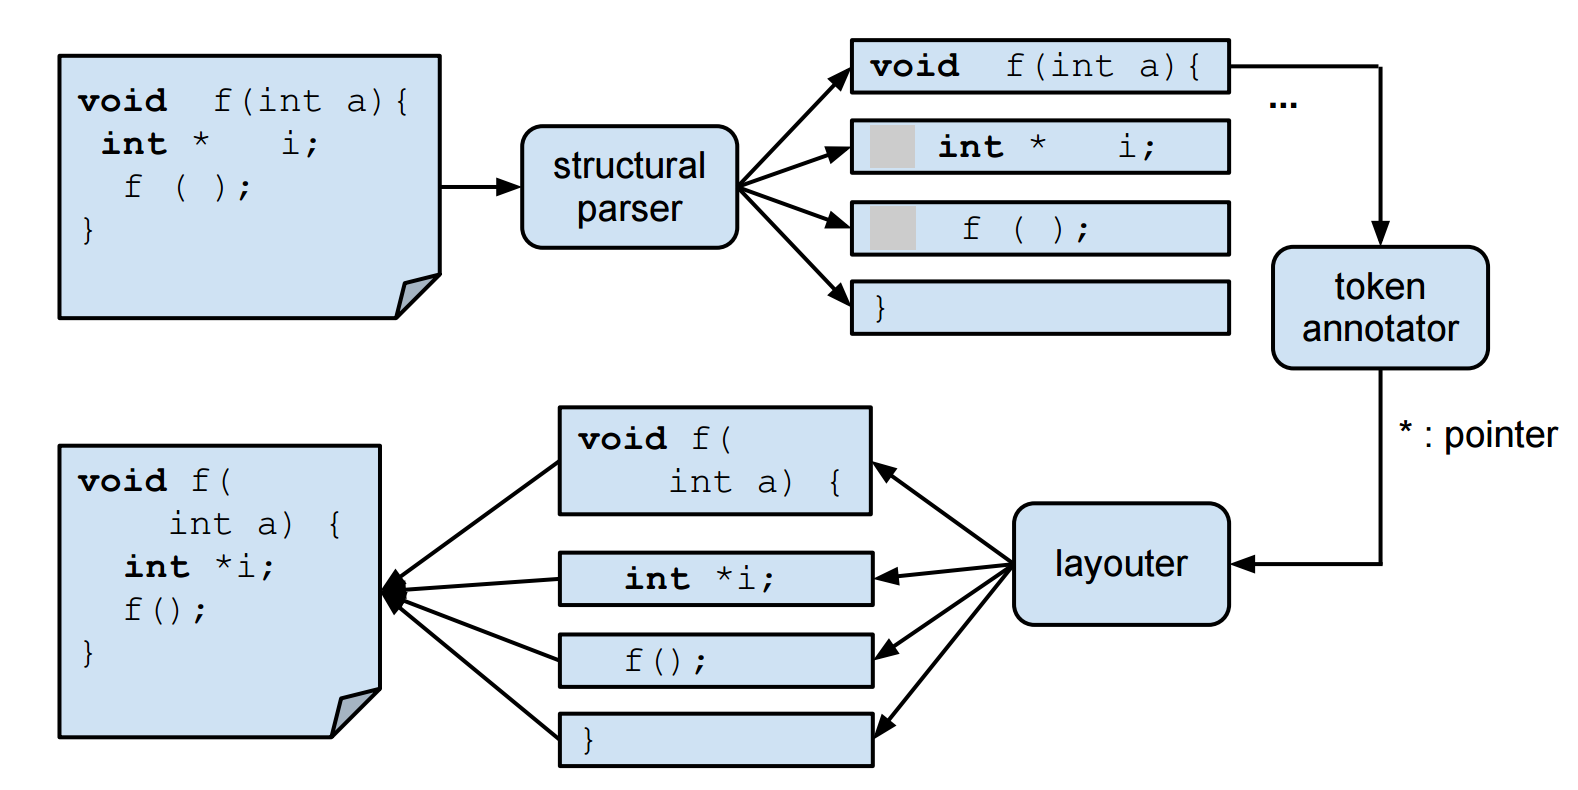
\includegraphics[width=0.9\textwidth]{img/clang-format.png}
  \caption{ClangFormat architecture}
  \label{fig:clang_format}
\end{figure}
The main components are the \emph{structural parser} and the \emph{layouter}.

ClangFormat employs a structural parser to split source code into a sequence of \emph{unwrapped-lines}.
An unwrapped line is a statement that should fit on a single line if given sufficient line length.
A key feature of unwrapped lines is that they should not influence other unwrapped lines.
The parser is lenient and parses even syntactically invalid code.
The parsed unwrapped lines are passed onto the layouter.

The ClangFormat layouter uses a novel approach to implement line wrapping.
Each line break is assigned a penalty according to several rules such as nesting and token type.
At each token, the layouter can choose to continue on the same line or break.
This forms an acyclic weighted directed graph with tokens representing vertices and splits (e.g., space, no space or line break) representing edges.
The first token of an unwrapped line is the root of the graph and all paths end at the last token of the unwrapped line.
The layouter uses Dijkstra's\autocite{dijkstra_note_1959} shortest path algorithm to find the layout that has the lowest penalty.
To obtain good performance, the layouter uses several domain specific optimizations to minimize the search space.

Despite supporting several programming languages, ClangFormat does not leverage the language agnostic formatting techniques described section~\ref{sec:agnostic}.
Support for each language has been added as ad-hoc extensions to the ClangFormat parser and layouter.
ClangFormat supports a variety of configuration options, including 6 out-of-the-box styles based on coding styles from Google, LLVM and other well-known organizations.

A notable feature of ClangFormat is that it's opinionated.
ClangFormat produces well-formatted output for even the most egregiously formatted input.
Listing~\ref{lst:clang_opinion} shows an offensively formatted C++ code snippet.
\lstinputlisting[label={lst:clang_opinion}, float, language=c, caption=Unformatted C++ code]{code/terrible.cpp}
Listing~\ref{lst:clang_opinion2} shows the same snippet after being formatted with ClangFormat.
\lstinputlisting[label={lst:clang_opinion2}, float, language=c, caption=ClangFormat formatted C++ code]{target/unterrible.cpp}
ClangFormat is opinionated because by default it does not respect the user's line breaking decisions.
This feature makes it possible to ensure that all code follows the same style guide, regardless of author.

\subsubsection{Dart}
Dartfmt\autocite{nystrom_dart_style_2014} was released in 2014 and follows the optimization based trend initiated by ClangFormat.
Dartfmt is a code formatter for the Dart programming language, developed at Google.
Like ClangFormat, dartfmt has a line length setting and is opinionated.
Bob Nystrom, the author of dartfmt, discusses the design of dartfmt in a blog post\autocite{nystrom_hardest_2015}.
In his post, Nystrom argues that the design of a code formatters is significantly complicated by a column limit setting.
The line wrapping algorithm in dartfmt employs a \emph{best-first search}\autocite{pearl_heuristics:_1984},
a minor variant of the shortest path search in ClangFormat.
As with ClangFormat, a range of domain-specific optimizations were required to make the search scale for real-world code.
Listing~\ref{lst:dead_end} shows an example of such an optimization, \emph{avoiding dead ends}.
\lstinputlisting[label={lst:dead_end}, float, caption=Avoid dead ends]{code/dead-end.dart}
The snippets exceeds the 35 character column limit.
A plain best-first search would perform a lot of redundant search inside the argument list of \texttt{firstCall}.
However, \texttt{firstCall} already fits on a line and there is no need to explore line breaks inside its argument list.
The dartfmt optimized search is able to eliminate such dead ends and quickly figure out to break before the \texttt{"long argument string"} literal.

\subsubsection{R}
The most recent addition to the optimization based formatting trend is \rfmt\autocite{yelland_new_2016},
a code formatter for the statistical programming environment \emph{R}.
The formatter was released in 2016 -- after the background work on this thesis started -- and like its forerunners is also developed at Google.
\rfmt{} makes an interesting contribution in that it combines the algebraic combinator approach from Hughes\autocite{hughes_design_1995} and the optimization based approach from \LaTeX{} and ClangFormat.

The algebraic combinator approach makes it easy to express a variety of formatting layouts.
\rfmt{} uses 6 layout combinators or \emph{blocks} as they are called in the report.
% , to express all formatting rules for the R programming language.
The blocks are the following:
\begin{itemize}
  \item $TextBlock(txt)$: unbroken string literal.
  \item $LineBlock(b_1, b_2, \ldots, b_n)$: horizontal combination of blocks.
  \item $StackBlock(b_1, b_2, \ldots, b_n)$: vertical combination of blocks.
  \item $ChoiceBlock(b_1, b_2, \ldots, b_n)$: selection of a best block.
  \item $IndentBlock(n, l)$: indent block $b$ by $n$ spaces.
  \item $WrapBlock(b_1, b_2, \ldots, b_n)$:
    Fit as many blocks on each line as possible, break when the column limit is exceeded and align by the first character in $b_1$.
    % Similar to \emph{bin-packing} in other code formatters such as ClangFormat.
\end{itemize}
We'll use an example to show how these relatively few combinators allow an impressive amount of flexibility.
Listings~\ref{lst:rfmt1} and~\ref{lst:rfmt2} shows two different layouts to format an argument list.

\begin{minipage}{.45\textwidth}
  \lstinputlisting[label={lst:rfmt1}, caption=Line block]{code/line.scala}
\end{minipage}
\hfil
\begin{minipage}{.45\textwidth}
  \lstinputlisting[label={lst:rfmt2}, caption=Stack block]{code/stack.scala}
\end{minipage}

In this case, we prefer the line block from listing~\ref{lst:rfmt1} since it requires fewer lines.
However, our preference changes if the function name is longer as is shown in listings~\ref{lst:rfmt3} and~\ref{lst:rfmt4}.

\begin{minipage}{.45\textwidth}
  \lstinputlisting[label={lst:rfmt3}, caption=Line block]{code/line1.scala}
\end{minipage}
\hfil
\begin{minipage}{.45\textwidth}
  \lstinputlisting[label={lst:rfmt4}, caption=Stack block]{code/stack1.scala}
\end{minipage}

Here, we clearly prefer the stack block in listing~\ref{lst:rfmt4}.
Listing~\ref{lst:rfmt-example} shows how we use the 6 fundamental blocks in the \rfmt{} combinator algebra to express the choice between these two formatting layouts.
\lstinputlisting[numbers=none, label={lst:rfmt-example},
                 caption=Formatting layout for argument lists]{code/rfmt-example.scala}
The variable $f$ denotes the function name and $a_1, ... a_m$ denotes the argument list.
Observe that listing~\ref{lst:rfmt-example} does not express how to find the optimal layout.

To find an optimal layout, \rfmt{} employs a novel indexing scheme.
First, it is possible enumerate all layout combinations like the re-predictor algorithm does in section~\ref{sec:lisp}.
This leads to exponential growth which turns out to be a problem for some cases.
Dynamic programming alleviates exponential growth by allowing us to reuse partial solutions.
Instead of re-calculating the layout cost at each (starting column, block) pair, we store the result in an associative array keyed by the starting column.
However, it turns out that this can still be inefficient in terms of memory and speed\footnote{
  In fact, ClangFormat started with a similar approach, as explained in this\autocite{clang84:online} video recording, but then switched to Dijkstra's shortest path algorithms (which in itself is another form of dynamic programming).
}.
To overcome this limitation, Yelland -- the \rfmt{} author -- presents an indexing scheme that makes it possible to extrapolate the layout cost even for missing keys.
We refer to the original paper\autocite{yelland_new_2016} for details.
This novel approach enables \rfmt{} to format even the most pathologically nested code in near instant time.

% TODO?
% \subsubsection{rustfmt} 

